% Options for packages loaded elsewhere
\PassOptionsToPackage{unicode}{hyperref}
\PassOptionsToPackage{hyphens}{url}
\PassOptionsToPackage{dvipsnames,svgnames,x11names}{xcolor}
%
\documentclass[
  letterpaper,
  DIV=11,
  numbers=noendperiod]{scrartcl}

\usepackage{amsmath,amssymb}
\usepackage{iftex}
\ifPDFTeX
  \usepackage[T1]{fontenc}
  \usepackage[utf8]{inputenc}
  \usepackage{textcomp} % provide euro and other symbols
\else % if luatex or xetex
  \usepackage{unicode-math}
  \defaultfontfeatures{Scale=MatchLowercase}
  \defaultfontfeatures[\rmfamily]{Ligatures=TeX,Scale=1}
\fi
\usepackage{lmodern}
\ifPDFTeX\else  
    % xetex/luatex font selection
\fi
% Use upquote if available, for straight quotes in verbatim environments
\IfFileExists{upquote.sty}{\usepackage{upquote}}{}
\IfFileExists{microtype.sty}{% use microtype if available
  \usepackage[]{microtype}
  \UseMicrotypeSet[protrusion]{basicmath} % disable protrusion for tt fonts
}{}
\makeatletter
\@ifundefined{KOMAClassName}{% if non-KOMA class
  \IfFileExists{parskip.sty}{%
    \usepackage{parskip}
  }{% else
    \setlength{\parindent}{0pt}
    \setlength{\parskip}{6pt plus 2pt minus 1pt}}
}{% if KOMA class
  \KOMAoptions{parskip=half}}
\makeatother
\usepackage{xcolor}
\setlength{\emergencystretch}{3em} % prevent overfull lines
\setcounter{secnumdepth}{5}
% Make \paragraph and \subparagraph free-standing
\makeatletter
\ifx\paragraph\undefined\else
  \let\oldparagraph\paragraph
  \renewcommand{\paragraph}{
    \@ifstar
      \xxxParagraphStar
      \xxxParagraphNoStar
  }
  \newcommand{\xxxParagraphStar}[1]{\oldparagraph*{#1}\mbox{}}
  \newcommand{\xxxParagraphNoStar}[1]{\oldparagraph{#1}\mbox{}}
\fi
\ifx\subparagraph\undefined\else
  \let\oldsubparagraph\subparagraph
  \renewcommand{\subparagraph}{
    \@ifstar
      \xxxSubParagraphStar
      \xxxSubParagraphNoStar
  }
  \newcommand{\xxxSubParagraphStar}[1]{\oldsubparagraph*{#1}\mbox{}}
  \newcommand{\xxxSubParagraphNoStar}[1]{\oldsubparagraph{#1}\mbox{}}
\fi
\makeatother


\providecommand{\tightlist}{%
  \setlength{\itemsep}{0pt}\setlength{\parskip}{0pt}}\usepackage{longtable,booktabs,array}
\usepackage{calc} % for calculating minipage widths
% Correct order of tables after \paragraph or \subparagraph
\usepackage{etoolbox}
\makeatletter
\patchcmd\longtable{\par}{\if@noskipsec\mbox{}\fi\par}{}{}
\makeatother
% Allow footnotes in longtable head/foot
\IfFileExists{footnotehyper.sty}{\usepackage{footnotehyper}}{\usepackage{footnote}}
\makesavenoteenv{longtable}
\usepackage{graphicx}
\makeatletter
\def\maxwidth{\ifdim\Gin@nat@width>\linewidth\linewidth\else\Gin@nat@width\fi}
\def\maxheight{\ifdim\Gin@nat@height>\textheight\textheight\else\Gin@nat@height\fi}
\makeatother
% Scale images if necessary, so that they will not overflow the page
% margins by default, and it is still possible to overwrite the defaults
% using explicit options in \includegraphics[width, height, ...]{}
\setkeys{Gin}{width=\maxwidth,height=\maxheight,keepaspectratio}
% Set default figure placement to htbp
\makeatletter
\def\fps@figure{htbp}
\makeatother
% definitions for citeproc citations
\NewDocumentCommand\citeproctext{}{}
\NewDocumentCommand\citeproc{mm}{%
  \begingroup\def\citeproctext{#2}\cite{#1}\endgroup}
\makeatletter
 % allow citations to break across lines
 \let\@cite@ofmt\@firstofone
 % avoid brackets around text for \cite:
 \def\@biblabel#1{}
 \def\@cite#1#2{{#1\if@tempswa , #2\fi}}
\makeatother
\newlength{\cslhangindent}
\setlength{\cslhangindent}{1.5em}
\newlength{\csllabelwidth}
\setlength{\csllabelwidth}{3em}
\newenvironment{CSLReferences}[2] % #1 hanging-indent, #2 entry-spacing
 {\begin{list}{}{%
  \setlength{\itemindent}{0pt}
  \setlength{\leftmargin}{0pt}
  \setlength{\parsep}{0pt}
  % turn on hanging indent if param 1 is 1
  \ifodd #1
   \setlength{\leftmargin}{\cslhangindent}
   \setlength{\itemindent}{-1\cslhangindent}
  \fi
  % set entry spacing
  \setlength{\itemsep}{#2\baselineskip}}}
 {\end{list}}
\usepackage{calc}
\newcommand{\CSLBlock}[1]{\hfill\break\parbox[t]{\linewidth}{\strut\ignorespaces#1\strut}}
\newcommand{\CSLLeftMargin}[1]{\parbox[t]{\csllabelwidth}{\strut#1\strut}}
\newcommand{\CSLRightInline}[1]{\parbox[t]{\linewidth - \csllabelwidth}{\strut#1\strut}}
\newcommand{\CSLIndent}[1]{\hspace{\cslhangindent}#1}

\usepackage{booktabs}
\usepackage{caption}
\usepackage{longtable}
\usepackage{colortbl}
\usepackage{array}
\usepackage{anyfontsize}
\usepackage{multirow}
\KOMAoption{captions}{tableheading}
\makeatletter
\@ifpackageloaded{caption}{}{\usepackage{caption}}
\AtBeginDocument{%
\ifdefined\contentsname
  \renewcommand*\contentsname{Table of contents}
\else
  \newcommand\contentsname{Table of contents}
\fi
\ifdefined\listfigurename
  \renewcommand*\listfigurename{List of Figures}
\else
  \newcommand\listfigurename{List of Figures}
\fi
\ifdefined\listtablename
  \renewcommand*\listtablename{List of Tables}
\else
  \newcommand\listtablename{List of Tables}
\fi
\ifdefined\figurename
  \renewcommand*\figurename{Figure}
\else
  \newcommand\figurename{Figure}
\fi
\ifdefined\tablename
  \renewcommand*\tablename{Table}
\else
  \newcommand\tablename{Table}
\fi
}
\@ifpackageloaded{float}{}{\usepackage{float}}
\floatstyle{ruled}
\@ifundefined{c@chapter}{\newfloat{codelisting}{h}{lop}}{\newfloat{codelisting}{h}{lop}[chapter]}
\floatname{codelisting}{Listing}
\newcommand*\listoflistings{\listof{codelisting}{List of Listings}}
\makeatother
\makeatletter
\makeatother
\makeatletter
\@ifpackageloaded{caption}{}{\usepackage{caption}}
\@ifpackageloaded{subcaption}{}{\usepackage{subcaption}}
\makeatother

\ifLuaTeX
  \usepackage{selnolig}  % disable illegal ligatures
\fi
\usepackage{bookmark}

\IfFileExists{xurl.sty}{\usepackage{xurl}}{} % add URL line breaks if available
\urlstyle{same} % disable monospaced font for URLs
\hypersetup{
  pdftitle={Comparing `Woody' and `Non-Woody' soil carbon distributions},
  pdfauthor={Ruan de Wet},
  colorlinks=true,
  linkcolor={blue},
  filecolor={Maroon},
  citecolor={Blue},
  urlcolor={Blue},
  pdfcreator={LaTeX via pandoc}}


\title{Comparing `Woody' and `Non-Woody' soil carbon distributions}
\author{Ruan de Wet}
\date{2025-01-03}

\begin{document}
\maketitle

\renewcommand*\contentsname{Table of contents}
{
\hypersetup{linkcolor=}
\setcounter{tocdepth}{3}
\tableofcontents
}

\section{Introduction}\label{introduction}

During the VCS validation audit for the VM0042 project titled
\href{https://registry.verra.org/app/projectDetail/VCS/2349}{Grassland
Restoration and Stewardship in South Africa (GRASS)}, a Forward Action
Request (FAR) was raised regarding the sampling applied to monitor soil
organic carbon stocks between rangelands of different tree densities
(greater and less than 10\% canopy cover). The wording of the FAR is
provided below:

\begin{quote}
VVB in the first verification will assess the stratified sampling
applied by PP for the parameter SOCbsl,i,t (Areal-average soil organic
carbon stocks in the baseline scenario for sample unit i in year t) to
check the sampling approach and its conservativeness. PP has proposed to
apply stratified random sampling in selecting sampling points to
distinguish between rangelands of different tree densities (greater and
less than 10\% canopy cover).
\end{quote}

Additional soil samples were collected in the 2023 sampling campaign to
address this FAR. Soil samples are grouped into strata from rangelands
with greater and with less than 10\% canopy cover - labelled `woody' and
`non-woody' strata, respectively.

\subsection{Sampling approach}\label{sampling-approach}

\subsubsection{Initial sampling
strategy}\label{initial-sampling-strategy}

Following the requirements of Section 8.6 of the VM0042 Methodology,
soil sampling sites were randomly assigned across the project accounting
area using \texttt{st\_sample()} from the \texttt{\{sf\}} package
(Pebesma 2018; Pebesma and Bivand 2023) in R (R Core Team 2024). This
generates a simple random sample of points within the defined spatial
features - the eligible grazing land within the active associations
under the GRASS project. Variation of the site location was allowed
based on field conditions within approximately 200 meters. This is to
account for unforeseen edge effects from foot paths, watering sites,
rocky outcrops, or any other factors that could skew the
representativeness of the samples collected from that site relative to
the surrounding landscape.

Initially, no distinction was made between grazing land with or without
tree cover and the only strata of interest were the implementation
landscapes (e.g.~uMkhomazi Catchment) to ensure that sufficient sampling
density was obtained within each landscape. Given that the statistical
power of the soil assessments are inversely correlated with the number
of strata, no further stratification was originally made within the
implementation landscapes.

The minimum target sampling density per landscape was one sample site
per 500 hectares. The field sampling team collected additional samples
beyond this minimum requirement at their discretion based on their
assessment of the variability of the topology, land use history, and
ecological context of the grazing lands.

\subsubsection{Defining eligible grazing
lands}\label{defining-eligible-grazing-lands}

An additional stratum was introduced with the raising of this FAR,
solely for the purposes of assessing whether any meaningful distinctions
exist across grazing lands of different tree densities (greater and less
than 10\% canopy cover).

This was necessitated because the
\href{https://verra.org/wp-content/uploads/2022/12/vcs-program-definitions-v4.3-final.pdf}{Verified
Carbon Standard (VCS) Program Definitions} defines ``Grasslands'' as
also including savannah ecosystems that have a mosaic of grass and tree
covers, which aligns with the latest ecological science on open
ecosystems (Bond 2019). The following description of a grassland is
provided:

\begin{quote}
Areas dominated by grasses with a density of trees too low to meet an
internationally accepted definition of forest, including savannas (i.e.,
grasslands with scattered trees). Grasslands also include managed
rangeland and pastureland that is not considered cropland where the
primary land use is grazing, and which may also include grass-dominated
systems managed for conservation or recreational purposes.
\end{quote}

Within the initial validation audit, a Corrective Action Request was
made by the reviewers with the expectation that a maximum woody cover
density threshold of 10\% should be applied as this is included in the
\href{https://www.fao.org/3/I8661EN/i8661en.pdf}{FAO definition} of a
forest. This definition, however, would exclude almost all definitions
of a savannah, which contradicts the
\href{https://verra.org/wp-content/uploads/2022/12/vcs-program-definitions-v4.3-final.pdf}{VCS
Program Definitions} that explicitly incorporate savannahs in the
definition of a grassland. Savannahs include a wide range of tree
densities that have been long described in southern Africa to exceed
10\% canopy cover density while still supporting grazing practices
(Edwards 1983).

The complexity of contradicting forest definitions has been addressed in
South Africa
\href{https://www.dffe.gov.za/sites/default/files/legislations/policyandguidelines_controlofdevelopmentaffecting_naturalforests.pdf}{through
legislation as well as in the South African court}. This is supported by
a technical definition that includes a largely contiguous canopy with a
cover threshold of 75\%, the dominance of trees, and the absence of
grasses and fire. This definition is consistent with the objective of
the VCS eligibility criteria, as it distinguishes forested land that is
not grazed (due to a lack of grass dominance) from treed savannahs that
\emph{are} grazed.

To assess whether or not additional stratification is required to
distinguish land that falls within the stricter definition of a savannah
(\textgreater10\% woody cover) from land that falls within a stricter
definition of a non-treed grassland (\textless10\% woody cover), soil
carbon measurements were collected across these strata. If statistically
significant difference in soil carbon concentrations can be detected
between sampling sites in the more woody cover relative to the less
woody land, this would suggest that further interrogation of the
monitoring plan may be justified and, perhaps, additional stratification
of the project area would be required.

The 2018 South African National Land Cover (SANLC) dataset was used to
distinguish between the strata. This dataset is developed, maintained
and distributed by the South African
\href{https://egis.environment.gov.za/\%20sa_national_land_cover_datasets}{Department
of Forestry, Fisheries, and the Environment (DFFE)}.

SANLC Classes 3, 4, and 42 are the only eligible land cover classes that
have \textgreater10\% woody canopy cover. Additional sampling sites were
randomly assigned within these land cover classes. The total extent of
these eligible woody classes account for approximately 8\%-10\% of the
total area, depending on the landscape.

\subsection{Analysis approach}\label{analysis-approach}

A two-sample t-test is used in this assessment to compare measured soil
carbon results across the two strata. The null hypothesis is tested that
the true difference in means between the two groups is equal to 0.

To determine the required sample size in the \texttt{Woody} stratum, a
power analysis has been run using the \texttt{pwr.t2n.test()} from the
\texttt{\{pwr\}} package (Champely 2020). This test takes as input the
existing sample size of the \texttt{Non-Woody} stratum, the standard
deviation of the same sample as the effect size, and calculates the
minimum required sample size of the \texttt{Woody} stratum to detect a
difference between the samples with a power of at least 0.5.

\begin{verbatim}

     t test power calculation 

             n1 = 198
             n2 = 40.93928
              d = 0.337854
      sig.level = 0.05
          power = 0.5
    alternative = two.sided
\end{verbatim}

To maximize the power of this analysis, more than 41 sites needed to be
sampled from the \texttt{Woody} stratum. Given that 64 sites were
sampled from the \texttt{Woody} stratum, it can be concluded that the
sample size was more than sufficient.

\section{Exploratory Data Analysis}\label{exploratory-data-analysis}

\subsection{Soil carbon data}\label{soil-carbon-data}

An initial visual exploration of the soil data will be helpful to
understand what the distributions look like.

\begin{table}

\caption{\label{tbl-soc-summary}}

\centering{

\caption*{
{\large Summary statistics for soil carbon (\%) across \texttt{woody} (\textgreater{}10\% cover) and \texttt{non-woody} (\textless{}10\% cover) strata.}
} 
\fontsize{12.0pt}{14.4pt}\selectfont
\begin{tabular*}{\linewidth}{@{\extracolsep{\fill}}lrrr}
\toprule
{\TEXTCOLOR[HTML]{A9A9A9}{GROUP}} & {\TEXTCOLOR[HTML]{A9A9A9}{COUNT}} & {\TEXTCOLOR[HTML]{A9A9A9}{MEAN}} & {\TEXTCOLOR[HTML]{A9A9A9}{SD}} \\ 
\midrule\addlinespace[2.5pt]
{Non-Woody} & {198} & {1.8520} & {1.4154} \\ 
{Woody} & {64} & {1.8679} & {1.2418} \\ 
\bottomrule
\end{tabular*}

}

\end{table}%

\begin{figure}

\centering{

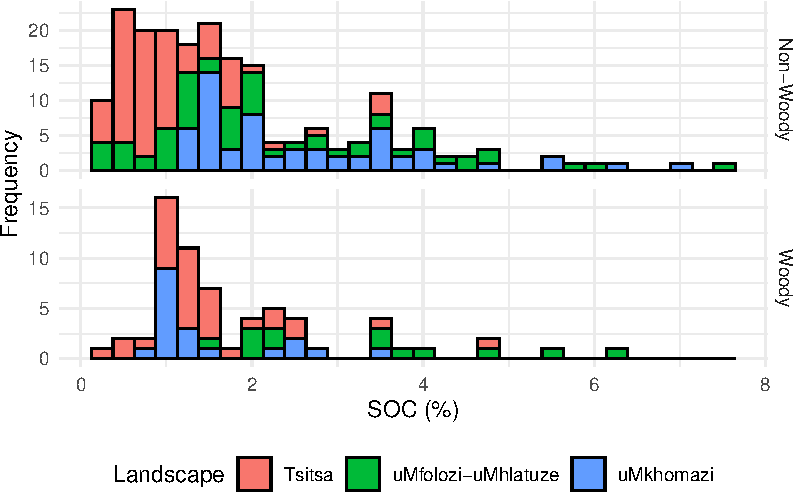
\includegraphics{woody-soil-carbon_files/figure-pdf/fig-soc-dist-1.pdf}

}

\caption{\label{fig-soc-dist}Soil carbon (\%) distribution across target
landscapes and \texttt{woody} (\textgreater10\% cover) and
\texttt{non-woody} (\textless10\% cover) strata.}

\end{figure}%

There is a considerable skew to the data, so a log10 transformation
might better represent the SOC data as a Gaussian response variable.

\begin{table}

\caption{\label{tbl-log10soc-summary}}

\centering{

\caption*{
{\large Summary statistics for log10-transformed soil carbon (\%) across \texttt{woody} (\textgreater{}10\% cover) and \texttt{non-woody} (\textless{}10\% cover) strata.}
} 
\fontsize{12.0pt}{14.4pt}\selectfont
\begin{tabular*}{\linewidth}{@{\extracolsep{\fill}}lrrr}
\toprule
{\TEXTCOLOR[HTML]{A9A9A9}{GROUP}} & {\TEXTCOLOR[HTML]{A9A9A9}{COUNT}} & {\TEXTCOLOR[HTML]{A9A9A9}{MEAN}} & {\TEXTCOLOR[HTML]{A9A9A9}{SD}} \\ 
\midrule\addlinespace[2.5pt]
{Non-Woody} & {198} & {0.1452} & {0.3379} \\ 
{Woody} & {64} & {0.1934} & {0.2561} \\ 
\bottomrule
\end{tabular*}

}

\end{table}%

\begin{figure}

\centering{

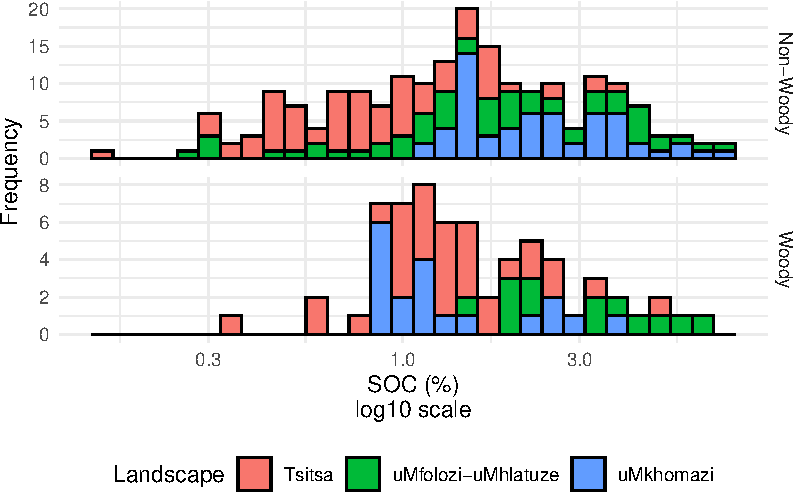
\includegraphics{woody-soil-carbon_files/figure-pdf/fig-log10soc-dist-1.pdf}

}

\caption{\label{fig-log10soc-dist}Log10-transformed soil carbon (\%)
distribution across target landscapes and \texttt{woody}
(\textgreater10\% cover) and \texttt{non-woody} (\textless10\% cover)
strata.}

\end{figure}%

\begin{figure}

\centering{

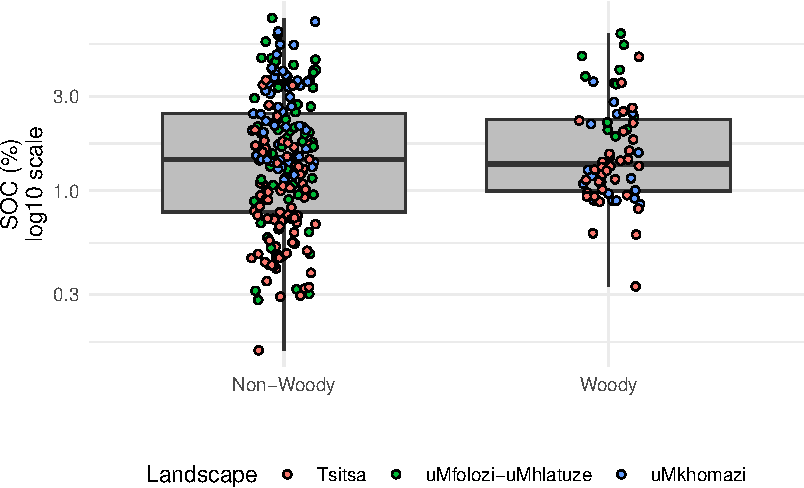
\includegraphics{woody-soil-carbon_files/figure-pdf/fig-log10soc-boxplots-1.pdf}

}

\caption{\label{fig-log10soc-boxplots}Log10-transformed soil carbon (\%)
boxplots across \texttt{woody} (\textgreater10\% cover) and
\texttt{non-woody} (\textless10\% cover) strata.}

\end{figure}%

\subsection{GRASS VCS Project
Boundary}\label{grass-vcs-project-boundary}

The first VCS monitoring period includes associations that joined the
GRASS project in 2021 and 2022. The boundary of the total area under
management for each association was mapped, but this includes a variety
of land cover classes that are ineligible for inclusion in the VCS
project. Details of the eligibility criteria and further exclusions that
were made go beyond the scope of this report and can be reviewed in the
GRASS validation audit documentation on the public
\href{https://registry.verra.org/app/projectDetail/VCS/2349}{Verra
registry}.

The \texttt{Woody} and \texttt{Non-Woody} strata are represented within
the eligible boundary areas.

\begin{table}

\caption{\label{tbl-lndscape-area}}

\centering{

\caption*{
{\large Total and eligible area (ha) across all landscapes represented in the first monitoring period.}
} 
\fontsize{12.0pt}{14.4pt}\selectfont
\begin{tabular*}{\linewidth}{@{\extracolsep{\fill}}>{\raggedright\arraybackslash}p{\dimexpr 112.50pt -2\tabcolsep-1.5\arrayrulewidth}>{\raggedleft\arraybackslash}p{\dimexpr 112.50pt -2\tabcolsep-1.5\arrayrulewidth}>{\raggedleft\arraybackslash}p{\dimexpr 112.50pt -2\tabcolsep-1.5\arrayrulewidth}}
\toprule
Landscape Name & Total area (ha) & Eligible area (ha) \\ 
\midrule\addlinespace[2.5pt]
{uMfolozi-uMhlatuze} & {33,301.93} & {27,346.82} \\ 
{uMkhomazi} & {26,092.19} & {18,081.98} \\ 
{Tsitsa} & {58,433.76} & {37,937.28} \\ 
\bottomrule
\end{tabular*}

}

\end{table}%

\subsection{Land cover data}\label{land-cover-data}

The
\href{https://egis.environment.gov.za/\%20sa_national_land_cover_datasets}{SANLC2018}
land cover classifications for all associations boundaries in the first
monitoring period have been extracted and summarized per landscape.

After excluding ineligible land cover, the remaining eligible classes
can be categorised as either \texttt{Woody} (classes 3, 4, and 42) and
\texttt{Non-Woody} (all other classes). The eligible \texttt{Woody}
classes account for 8\%-10\% of the total land cover, depending on the
landscape.

\begin{table}

\caption{\label{tbl-sanlc-strata}}

\centering{

\caption*{
{\large Eligible South African National Land Cover (SANLC) classes occuring across GRASS associations and their assignment to \texttt{Woody} and \texttt{Non-Woody} strata.}
} 
\fontsize{12.0pt}{14.4pt}\selectfont
\begin{tabular*}{\linewidth}{@{\extracolsep{\fill}}l|rl}
\toprule
 & {\TEXTCOLOR[HTML]{A9A9A9}{CLASS}} & Class Name \\ 
\midrule\addlinespace[2.5pt]
\multirow{3}{*}{Woody} & {3} & {Dense Forest \& Woodland (35 - 75\% cc)} \\ 
 & {4} & {Open Woodland (10 - 35\% cc)} \\ 
 & {42} & {Fallow Land \& Old Fields (Trees)} \\ 
\midrule\addlinespace[2.5pt]
\multirow{8}{*}{Non-Woody} & {8} & {Low Shrubland (other regions)} \\ 
 & {13} & {Natural Grassland} \\ 
 & {27} & {Eroded Lands} \\ 
 & {31} & {Other Bare} \\ 
 & {43} & {Fallow Land \& Old Fields (Bush)} \\ 
 & {44} & {Fallow Land \& Old Fields (Grass)} \\ 
 & {45} & {Fallow Land \& Old Fields (Bare)} \\ 
 & {46} & {Fallow Land \& Old Fields (Low Shrub)} \\ 
\bottomrule
\end{tabular*}

}

\end{table}%

The simple random site allocation for sampling within the \texttt{Woody}
stratum ensures that the samples are representative. Given that the
\texttt{Non-Woody} stratum accounts for a much larger extent of the
eligible land than the \texttt{Woody} stratum (\textasciitilde90/10),
equal sampling efforts across both strata result in an unequal sample
size. Additional sites were, therefore, sampled to increase the
\texttt{Woody} stratum sample size and improve the sample ratio
(\textasciitilde70/30).

\begin{figure}

\centering{

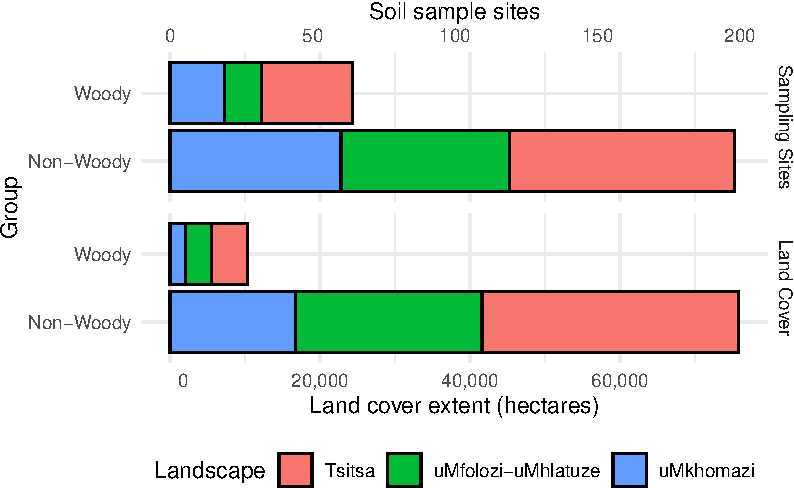
\includegraphics{woody-soil-carbon_files/figure-pdf/fig-sanlc-woody-1.pdf}

}

\caption{\label{fig-sanlc-woody}Eligible land cover extent (ha) and
number of soil sampling sites between \texttt{woody} (\textgreater10\%
cover) and \texttt{non-woody} (\textless10\% cover) strata across the
relevant landscapes.}

\end{figure}%

\section{Parametric Test Assumptions}\label{parametric-test-assumptions}

In order to apply a parametric t-test, the data should be Gaussian
(normally distributed) and homoscedastic (equal variance). If these
assumptions are violated, then an alternative test, such as the Welch
t-test, may be required.

This
\href{http://www.sthda.com/english/wiki/unpaired-two-samples-t-test-in-r}{STHDA
article} provides more information on the steps followed in this
analysis.

\subsection{Normal distribution}\label{normal-distribution}

A visual inspection of the log10-transformed SOC data indicates that the
data are normally distributed. The Shapiro-Wilk normality test can be
used to test this more quantitatively. The null hypothesis is that the
data are normal. If p-value \textgreater{} 0.05, then the data are not
significantly different from normal.

\begin{verbatim}

    Shapiro-Wilk normality test

data:  SOC_log10[Group == "Non-Woody"]
W = 0.9884, p-value = 0.1072
\end{verbatim}

\begin{verbatim}

    Shapiro-Wilk normality test

data:  SOC_log10[Group == "Woody"]
W = 0.96643, p-value = 0.07873
\end{verbatim}

For both ``Woody'' and ``Non-Woody'' data, the p-values are
\textgreater{} 0.05. We can therefore assume normality for both
datasets.

\subsection{Equal variance}\label{equal-variance}

The homogeneity in variances of the two groups can be tested with an
F-test. The null hypothesis is that the ratio of variances is equal to
1.

\begin{verbatim}

    F test to compare two variances

data:  SOC_log10 by Group
F = 1.7401, num df = 197, denom df = 63, p-value = 0.01134
alternative hypothesis: true ratio of variances is not equal to 1
95 percent confidence interval:
 1.137268 2.551662
sample estimates:
ratio of variances 
          1.740069 
\end{verbatim}

The p-value is \textless{} 0.05. We can therefore reject the null
hypothesis and infer that the ratio of variances are not equal to 1. The
data have therefore failed the test of equal variance and a
non-parametric two-sample t-test (Welch t-test) needs to be applied.

\subsection{Welch two-sample t-test}\label{welch-two-sample-t-test}

The null hypothesis of the t-test is that the true difference in means
between the two groups is equal to 0. There's no prior expectation that
one group would be greater or less than the other, so a two-sided
hypothesis is applied by default.

\begin{verbatim}

    Welch Two Sample t-test

data:  SOC_log10 by Group
t = -1.2051, df = 139.67, p-value = 0.2302
alternative hypothesis: true difference in means between group Non-Woody and group Woody is not equal to 0
95 percent confidence interval:
 -0.12734721  0.03089267
sample estimates:
mean in group Non-Woody     mean in group Woody 
              0.1452139               0.1934412 
\end{verbatim}

\section{Conclusion}\label{conclusion}

The p-value is \textgreater{} 0.05, so the null hypothesis cannot be
rejected, and it can be concluded that \textbf{\emph{there is no
difference in SOC between the \texttt{Woody} and \texttt{Non-Woody}
strata}}.

\phantomsection\label{refs}
\begin{CSLReferences}{1}{0}
\bibitem[\citeproctext]{ref-bond-2019}
Bond, William J. 2019. {``Open Ecosystems: Ecology and Evolution Beyond
the Forest Edge,''} July.
\url{https://doi.org/10.1093/oso/9780198812456.001.0001}.

\bibitem[\citeproctext]{ref-pwr-2020}
Champely, Stephane. 2020. \emph{Pwr: Basic Functions for Power
Analysis}. \url{https://CRAN.R-project.org/package=pwr}.

\bibitem[\citeproctext]{ref-edwards-1983}
Edwards, E. 1983. {``A Broad-Scale Structural Classification of
Vegetation for Practical Purposes.''} \emph{Bothalia} 14 (3/4): 705--12.
\url{https://doi.org/10.4102/abc.v14i3/4.1231}.

\bibitem[\citeproctext]{ref-pebesma-2018}
Pebesma, Edzer. 2018. {``{Simple Features for R: Standardized Support
for Spatial Vector Data}.''} \emph{{The R Journal}} 10 (1): 439--46.
\url{https://doi.org/10.32614/RJ-2018-009}.

\bibitem[\citeproctext]{ref-pebesma-bivand-2023}
Pebesma, Edzer, and Roger Bivand. 2023. \emph{{Spatial Data Science:
With applications in R}}. {Chapman and Hall/CRC}.
\url{https://doi.org/10.1201/9780429459016}.

\bibitem[\citeproctext]{ref-RManual}
R Core Team. 2024. \emph{R: A Language and Environment for Statistical
Computing}. Vienna, Austria: R Foundation for Statistical Computing.
\url{https://www.R-project.org/}.

\end{CSLReferences}




\end{document}
